\documentclass{bioinfo}
\copyrightyear{2019}
\pubyear{2019}

% \usepackage{hyperref}
\usepackage{url}
\usepackage{amsmath}
\usepackage{array}
\usepackage{booktabs}
\usepackage[normalem]{ulem}
\usepackage{xcolor}
%\usepackage{lmodern}

\usepackage{xspace}
\def\etal{{\em et al.}\xspace}

\usepackage{listings}
\usepackage{color}

\definecolor{dkgreen}{rgb}{0,0.6,0}
\definecolor{gray}{rgb}{0.5,0.5,0.5}
\definecolor{mauve}{rgb}{0.58,0,0.82}

\newcommand{\opentsne}[0]{{\tt openTSNE}\ }

\lstset{
  frame=none,
  % frame=tb,
  numbers=none, % left
  language=Python,
  aboveskip=1mm,
  belowskip=1mm,
  showstringspaces=false,
  columns=flexible,
  basicstyle={\small\ttfamily},
  numberstyle=\tiny\color{gray},
  keywordstyle=\color{blue},
  commentstyle=\color{dkgreen},
  stringstyle=\color{dkgreen},
  breaklines=true,
  breakatwhitespace=true,
  tabsize=3
}


\providecommand{\e}[1]{\ensuremath{\times 10^{#1}}}
\setlength{\textfloatsep}{11pt}

\access{Advance Access Publication Date: Day Month Year}
\appnotes{Data and text mining}

% Applications notes: Title page, Short Structured Abstract, Text.
\begin{document}
\firstpage{1}

\subtitle{Data and text mining}

\title[openTSNE: a modular Python library for t-SNE dimensionality reduction and embedding]{openTSNE: a modular Python library for t-SNE dimensionality reduction and embedding}
\author[Poli\v{c}ar \textit{et~al}.]{
  Pavlin G. Poli\v{c}ar\,$^{\text{\sfb 1,}*}$
  Martin Stra\v{z}ar\,$^{\text{\sfb 1}}$
  and
  Bla\v{z} Zupan\,$^{\text{\sfb 1, 2}}$}
\address{
$^{\text{\sf 1}}$Faculty of Computer and Information Science, University of Ljubljana, SI-1000 Ljubljana, Slovenia, \\
$^{\text{\sf 2}}$Department of Molecular and Human Genetics, Baylor College of Medicine, Houston TX 77030, U.S.A.
}

\corresp{$^\ast$To whom correspondence should be addressed.}

\history{Received on N/A; revised on N/A; accepted on N/A}

\editor{Associate Editor: TBA}

\abstract{\textbf{Summary:}
Point-based visualisations of large, multi-dimensional data from
molecular biology can reveal structures and clusters. One of the
most popular techniques to construct such visualisations is t-distributed
stochastic neighbor embedding (t-SNE), for which a number of extensions have
recently been proposed to address speed and quality of the resulting
visualisations. We propose openTSNE, a modular Python library that implements
the core t-SNE algorithm and its extensions. The library is orders of magnitude
faster than existing popular implementations, including those from
scikit-learn. Unique to openTSNE is also the mapping of new data to an existing embedding, which
can surprisingly assist in solving batch effect problems.
\\
\textbf{Availability:} openTSNE is available at \url{https://github.com/pavlin-policar/openTSNE}.\\
\textbf{Contact:} \href{pavlin.policar@fri.uni-lj.si}{pavlin.policar@fri.uni-lj.si}\\
% \textbf{Supplementary information:} Supplementary data are available at \textit{Bioinformatics} online.
}

\maketitle



The abundance of high-dimensional data sets in molecular biology calls for
techniques for dimensionality reduction, and in particular for methods that can
help in the construction of data visualizations. Popular approaches for
dimensionality reduction include principal component analysis, multidimensional
scaling, and uniform manifold approximation and projections~\citep{umap}. Among
these, t-distributed stochastic neighbor embedding
(t-SNE)~\citep{tsne} lately received much attention as it can
address high volumes of data and reveal clustering structure. Most
of the recent reports on single-cell gene expression data would start with an
overview of the cell landscape, where t-SNE embeds high-dimensional expression
profiles into two dimensional space~\citep{Macosko2015, Shekhar2016}.
Fig.~\ref{fig:tsne}.a presents an example of such an embedding.

Despite its utility, t-SNE has lately been criticized for insufficient speed
when addressing huge data sets, lack of global organization \em t-SNE
focuses on local clusters that are then arbitrarily scattered in the
low-dimensional space \em and absence of theoretically-founded implementations to
map new data into an existing embedding. Most of these shortcomings, however, were
recently addressed~\citep{ding2018interpretable,becht2019dimensionality}.
\citet{fi_tsne} sped-up the method through interpolation-based
approximation, reducing the time complexity to be merely linear
in the number of data items. \citet{art_of_using_tsne} proposed
several techniques to improve global positioning, including estimating similarities with a mixture of
Gaussian kernels. While no current popular
software library supports mapping of new data into reference embedding,
\citet{parametric_tsne} proposed a related approach with parametric mapping
using neural networks.

We here introduce \opentsne, a comprehensive Python library that
implements t-SNE with all recently proposed extensions. The library is
compatible with Python data science ecosystem (e.g., {\tt numpy}, {\tt
sklearn}, {\tt scanpy}). Its modular design fosters extendibility and
experimentation with various setting and changes in the analysis pipeline. For
example, the following code uses multiscale similarity kernels to construct the
embedding from Fig.~\ref{fig:tsne}.b.

\begin{lstlisting}
adata = anndata.read_h5ad("macosko_2015.h5ad")
affinities = openTSNE.affinity.Multiscale(
	adata.obsm["pca"], perplexities=[50, 500], metric="cosine")
init = openTSNE.initialization.pca(adata.obsm["pca"])
embedding = TSNEEmbedding(init, affinities)
embedding.optimize(n_iter=250, exaggeration=12, momentum=0.5, inplace=True)
embedding.optimize(n_iter=750, momentum=0.8, inplace=True)
\end{lstlisting}

\noindent Here, we first read the data, define the affinity model based on two
Gaussian kernels with varying perplexity, use a PCA-based initialization, and run
the typical two-stage t-SNE optimization. Notice that the code for the standard
t-SNE used for Fig.~\ref{fig:tsne}.a is similar but uses only a single kernel
({\tt perplexities=[30]}).

\begin{figure}[htbp]
\centerline{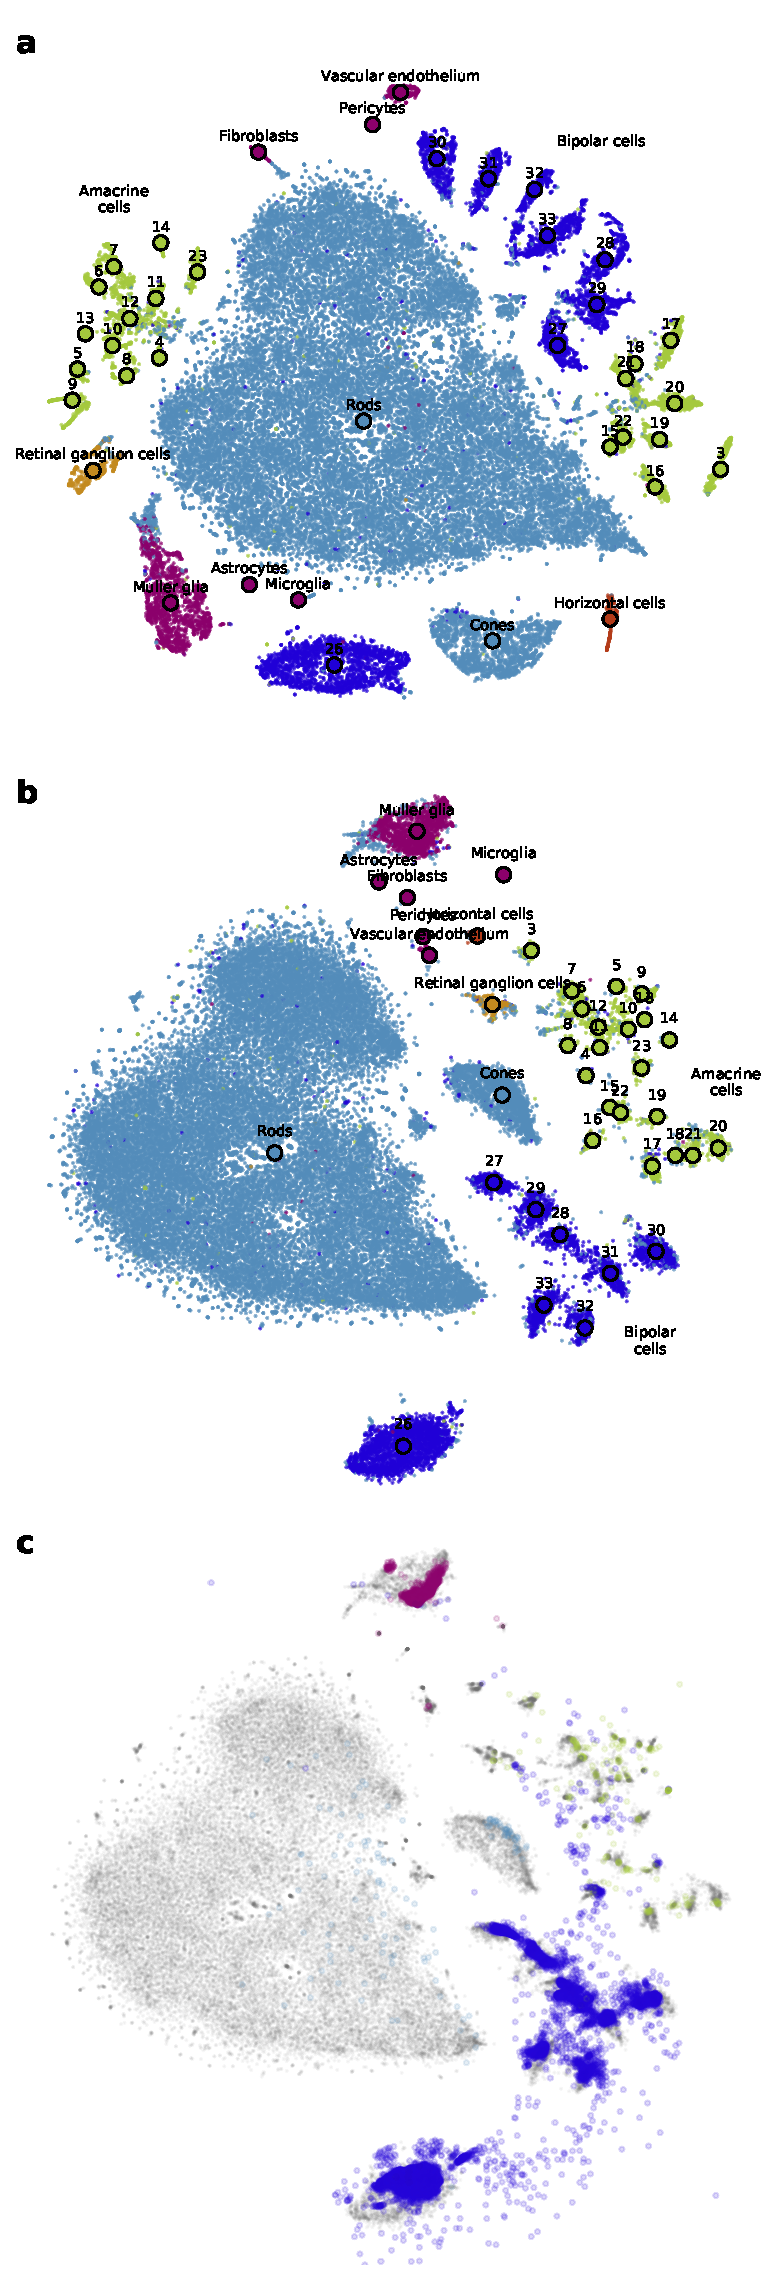
\includegraphics[width=0.7\linewidth]{policar-fig-1}}
\caption{Example application of \opentsne on mouse retina cells from
\citet{Macosko2015} and \citet{Shekhar2016}. a) Standard t-SNE embedding using
random initialization and perplexity of 30. b) t-SNE embedding using
multi-scale affinities leads to better global cluster organization. Cluster
annotations in both a) and b) are from Macosko~\etal c) Embedding of independent mouse retina cells from
Shekhar~\etal (points in color) to a reference t-SNE visualization of data from
Macosko~\etal (points in gray) places cells in the clusters that match
classifications from original publications and alleviates batch effects.}
\label{fig:tsne}
\end{figure}

The proposed \opentsne library is currently the only Python t\nobreakdash -SNE
implementation that supports adding new samples into constructed embedding. For
example, we can reuse the {\tt embedding} created above to map new data into
existing embedding space in the following code,

\begin{lstlisting}
new_data = anndata.read_h5ad("shekhar_2016.h5ad")
adata, new_data = find_shared_genes(adata, new_data)
gene_mask = select_genes(adata.X, n=1000)
embedding.affinities = affinity.PerplexityBasedNN(
	adata[:, gene_mask].X, perplexity=30, metric="cosine")
new_embedding = embedding.transform(
	new_data[:, gene_mask].X)
\end{lstlisting}

\noindent which loads and prepare the new data, defines the affinity model, and
computes the embeddings. \opentsne embeds new data one data instance at the
time, without changing the reference embedding. The example of combining two
data sets with mouse retina cells is shown on Fig.~\ref{fig:tsne}.c, where the
cells of the secondary data set get matched to the cells in the reference
embedding. This
procedure can therefore be used for handling batch effects~\citep{polivcar2019embedding}, a substantial
problem in molecular biology when dealing with the data from different
sources~\citep{batch_effect_causes}. The code for plotting of the data is not shown
for brevity, but is, together with other examples, available on {\opentsne}'s
GitHub page. 

Our Python implementation introduces computational overhead: \opentsne is about
25\% slower than {\tt FIt-SNE}~\citep{fi_tsne}, a recent t-SNE implementation
in C++. However, \opentsne is still orders of magnitude faster than other
Python implementations, including those from {\tt scikit-learn} and {\tt
MulticoreTSNE} (see Benchmarks in \opentsne documentation on GitHub). An example data sets with 200,000 cells
is processed in more than 90 minutes with scikit-learn and less than 4 minutes with \opentsne.
The framework includes controlled execution (callback-based progress monitoring and
control), making it suitable for interactive data exploration environments such
as Orange~\citep{scorange}. Pure Python implementation offers distinct
advantages that include integration with Python's rich data science
infrastructure and ease of installation through PyPI and {\em conda}.

\section*{Funding and Acknowledgements}
The support for this work was provided by the Slovenian Research Agency Program
Grant P2-0209, and by European Regional Development Fund and the Slovenian
Ministry of Education through BioPharm project. We want to thank George
Linderman and Dmitry Kobak for helpful discussions on extensions of t-SNE.

\bibliographystyle{natbib}
\bibliography{policar.bib}
% \end{document}

% \begin{thebibliography}{}
% \end{thebibliography}



\end{document}
